\chapter{Evaluation}
\label{sec:evaluation}
\minitoc
\vspace*{1cm}

and the way
we deployed our WordPress application using containers to
evaluate our fuzzer's performance.

% NEW SECTION
\section{Methodology}
For the evaluation of our tool, we opted for convenience to use Docker ~\cite{docker_def}, which we also discussed in Chapter ~\ref{sec:background}. Docker is a software that can package your application, its dependencies, system tools, system libraries and settings in a single comprehensive virtual container. This is because Docker is lightweight, portable and can improve application development and deployment considerably. As we already mentioned in Chapter ~\ref{sec:architecture}, \pname{} is limited to web applications written in PHP due to the instrumentation. What are the best web applications to evaluate our tool on?

The WordPress CMS (Content Management System) ~\cite{docker_def} is one of the most popular open-source web application for managing and publishing content on the web, with nearly half of the top 1 million sites on the internet using it. While it powers more than a third of the web, what is more important about it, for us, is that it is written in PHP and widely used for building a variety of websites, ranging from simple blog spots to professional web sites. We tested our tool on second web application, Drupal CMS ~\cite{drupal}. Drupal is a free and open-source content-management framework written in PHP and distributed under the GNU General Public License. It is used as a back-end framework for at least 2.1\% of all Web sites worldwide ranging from personal blogs to corporate, political, and government sites.

Using Docker, and more specifically its docker-compose functionality, we where able to achieved a multi-container deployment through a single docker-compose YAML file for the following services:

\begin{itemize}
	\item {\tt NGINX }: An open-source, high-performance HTTP server which handles all the HTTP request made by \pname{} and forwarded to our WordPress or Drupal web applications.{~\cite{nginx}}
	\item {\tt WordPress and Drupal }: Both open-source CMS web application. Since having access to the code, we began by examining the existing system in terms of injecting bugs and performing our instrumentation.
	\item {\tt MariaDB }: A popular open source relational databases which we used to store and manipulate the WordPress data~\cite{mariadb}.
\end{itemize}

The official images for the above services can be found for free at Docker Hub. An illustration of the above infrastructure in the case of WordPress, can be viewed at Figure ~\ref{fig:multi-container}. Files and instructions for replicating this process can be found at the fuzzer's repository.

\begin{figure}[ht]
 \centering
 \captionsetup{justification=centering}
 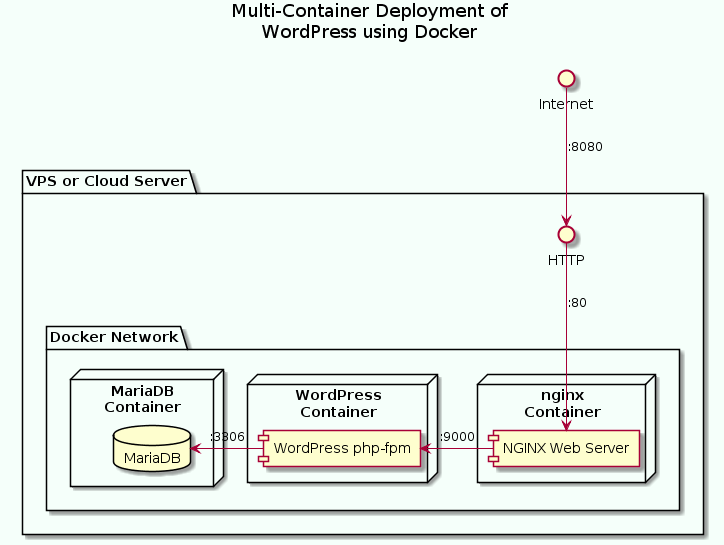
\includegraphics[width=\linewidth]{figures/multi-container.png}
 \caption{Evaluation followed the above Multi-Container Deployment of WordPress using Docker ~\cite{multi-container}.}
 \label{fig:multi-container}
\end{figure}

\section{Automated Vulnerability Addition}
